\documentclass[11pt,a4paper]{article}
\usepackage[textwidth=37em,vmargin=30mm]{geometry}
\usepackage{calc,xunicode,amsmath,amssymb,paralist,enumitem,tabu,booktabs,datetime2,xeCJK,xeCJKfntef,listings}
\usepackage{tocloft,fancyhdr,tcolorbox,xcolor,graphicx,eso-pic}

\usepackage[hidelinks]{hyperref}
\hypersetup{
    colorlinks=false,
    pdfpagemode=FullScreen,
    pdftitle={Web Digest - 2023-01-07}
}

\setdefaultleftmargin{2em}{2em}{1em}{1em}{1em}{1em}

\usepackage{xeCJK,xeCJKfntef}
\newcommand{\myvphantom}[0]{\vphantom{QWERTYUIOPASDFGHJKLZXCVBNMqwertyuiopasdfghjklzxcvbnm1234567890ςρθδφγηξλζχψβμ\"A}}
\xeCJKsetup{PunctStyle=plain,RubberPunctSkip=false,CJKglue=\myvphantom\hskip 0pt plus 0.1em minus 0.05em,CJKecglue=\myvphantom\hskip 0.22em plus 200pt}
\XeTeXlinebreaklocale "zh"
\XeTeXlinebreakskip = 0pt


\setmainfont[Numbers=Lining]{Brygada 1918}
\setromanfont[Numbers=Lining]{Brygada 1918}
\setsansfont[Numbers=Lining]{IBM Plex Sans}
\setmonofont{JetBrains Mono NL}
\setCJKmainfont{Noto Serif CJK SC}
\setCJKromanfont{Noto Serif CJK SC}
\setCJKsansfont{Noto Sans CJK SC}
\setCJKmonofont{Noto Sans CJK SC}

\setlength{\parindent}{0pt}
\setlength{\parskip}{8pt}
\linespread{1.15}

\lstset{
	basicstyle=\ttfamily\footnotesize,
	numbersep=5pt,
	backgroundcolor=\color{black!5},
	showspaces=false,
	showstringspaces=false,
	showtabs=false,
	tabsize=2,
	captionpos=b,
	breaklines=true,
	breakatwhitespace=true,
	breakautoindent=true,
	linewidth=\textwidth
}






\newcommand{\coverpic}[2]{
    % argv: itemurl, authorname
    Cover photo by #2~~~~(\href{#1}{#1})
}
\newcommand{\makeheader}[0]{
    \begin{center}
        
        \rmfamily\scshape
        \fontsize{62pt}{70pt}\selectfont
        WEB\hfill DIGEST
        
        \vfill
        % \vskip 30pt
        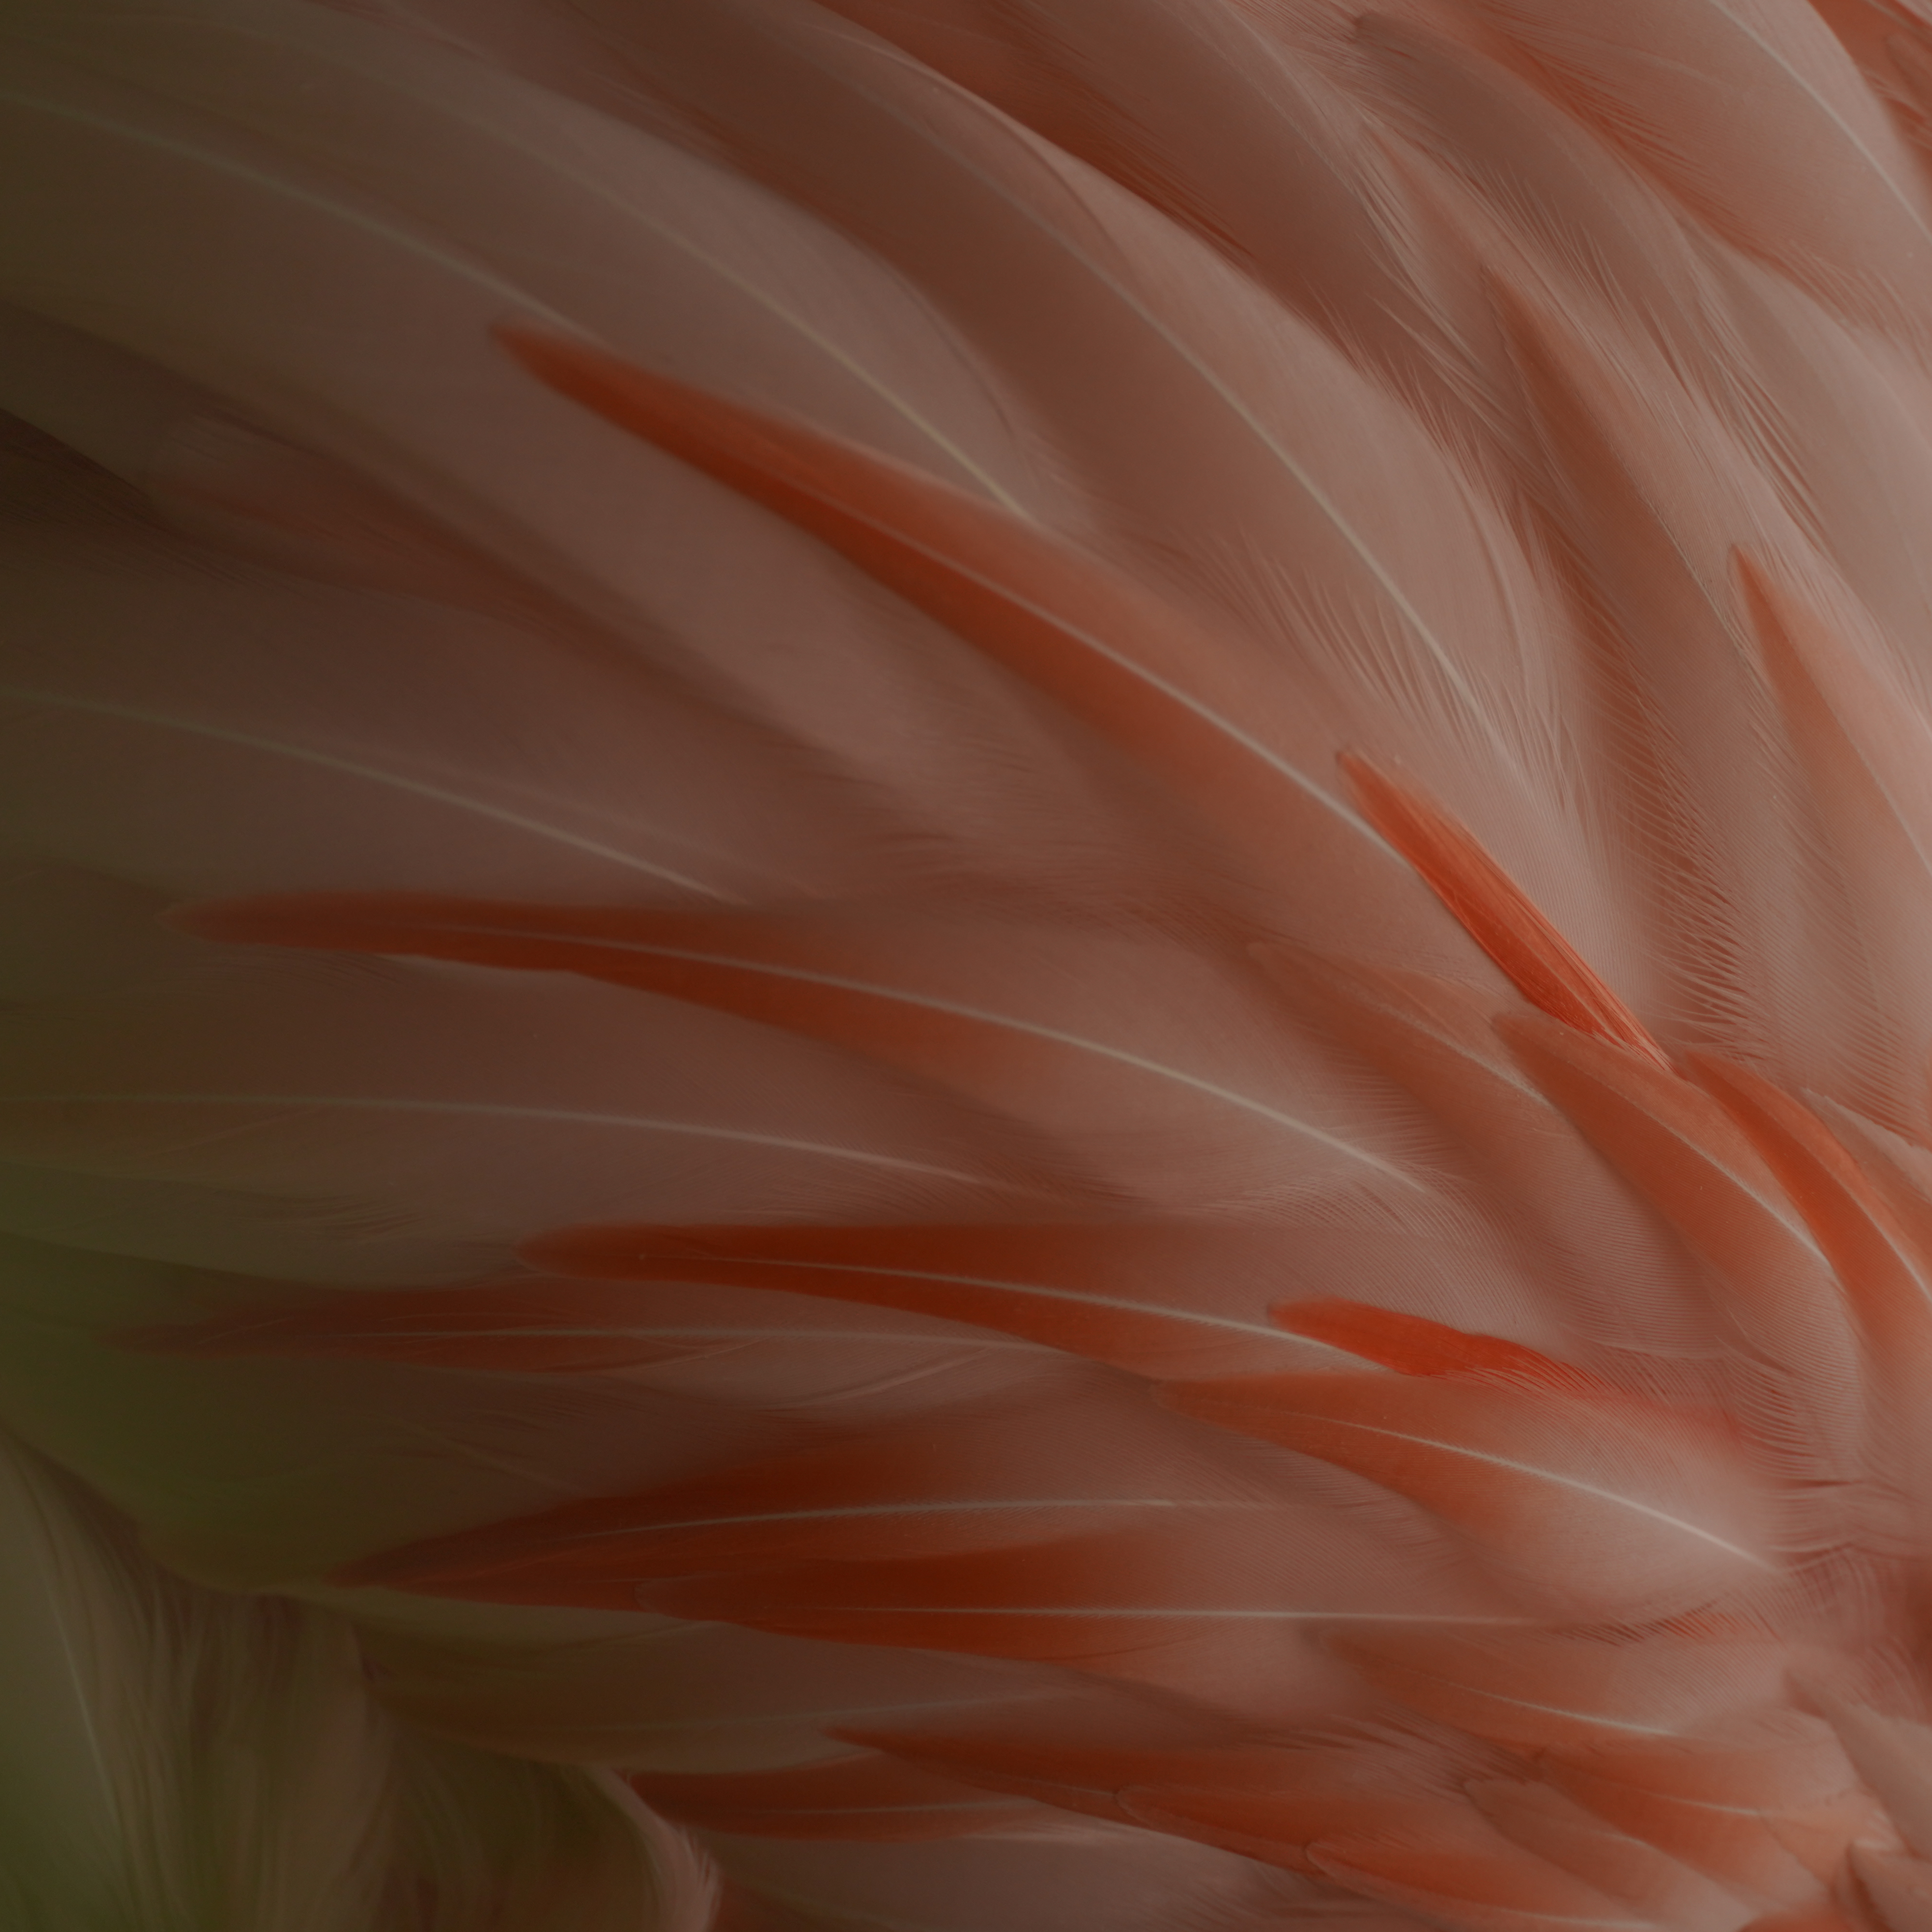
\includegraphics[width=\linewidth]{./webdb/20230107/final/coverpic.jpg}\par
        % \vskip 30pt
        \vfill

        \normalsize\upshape
        \copyright{} The Web Digest Project \hfill\large 2023-01-07
    \end{center}
    % \vskip 20pt
    % \hrule
    % \vskip 10pt
    % \clearpage
}
\renewcommand{\contentsname}{\Huge\sffamily\bfseries Contents\par\vskip 20pt}
\newcounter{ipartcounter}
\setcounter{ipartcounter}{0}
\newcommand{\ipart}[1]{
    % \vskip 20pt
    \clearpage
    \stepcounter{ipartcounter}
    \phantomsection
    \addcontentsline{toc}{section}{#1}
    \begin{center}
        \Huge
        \sffamily\bfseries
        #1
    \end{center}
    \vskip 20pt
}
\newcommand{\entryitemHackernews}[3]{
    % argv: title, hnurl, rawurl
    \parbox{\linewidth}{
        \Large\rmfamily\bfseries#1\par\vskip 5pt
        \footnotesize\ttfamily\mdseries
        \href{#3}{#3}\par
        \textcolor{black!50}{\href{#2}{#2}}\par
    }\vskip 11pt
}
\newcommand{\entryitemGeneric}[2]{
    % argv: title, url
    \parbox{\linewidth}{
        \Large\rmfamily\bfseries#1\par\vskip 5pt
        \footnotesize\ttfamily\mdseries
        \href{#2}{#2}\par
    }\vskip 11pt
}






\begin{document}

\begin{titlepage}
	\makeheader
\end{titlepage}

\tableofcontents\clearpage


\ipart{Hacker News}
\entryitemTwoLinks{Using your Kindle as an e-ink monitor}{https://news.ycombinator.com/item?id=41155177}{https://gist.github.com/adtac/eb639d3c707b55a28f0ee9a420aa7e0c}

\entryitemTwoLinks{WhenFS: Calender Is Now a File System}{https://news.ycombinator.com/item?id=41154616}{https://github.com/lvkv/whenfs}

\entryitemTwoLinks{Jailbroke my Kindle to use it as an e-ink monitor}{https://news.ycombinator.com/item?id=41154410}{https://gist.github.com/adtac/eb639d3c707b55a28f0ee9a420aa7e0c}

\entryitemTwoLinks{Porting My JavaScript Game Engine to C for No Reason}{https://news.ycombinator.com/item?id=41154135}{https://phoboslab.org/log/2024/08/high\_impact}

\entryitemTwoLinks{Written by a 16 year old, a book on how computers work}{https://news.ycombinator.com/item?id=41153892}{https://github.com/hackclub/RAM-a-thon}

\entryitemTwoLinks{Belenios: Verifiable online voting system}{https://news.ycombinator.com/item?id=41153158}{https://www.belenios.org/}

\entryitemTwoLinks{The Untold Story of How US Spies Sabotaged Soviet Technology}{https://news.ycombinator.com/item?id=41153093}{https://www.politico.com/news/magazine/2024/08/04/us-spies-soviet-technology-00164126}

\entryitemTwoLinks{Self-Compressing Neural Networks}{https://news.ycombinator.com/item?id=41153039}{https://arxiv.org/abs/2301.13142}

\entryitemTwoLinks{Organic maps: Experimental feed based public transport mapping}{https://news.ycombinator.com/item?id=41152559}{https://github.com/organicmaps/organicmaps/blob/master/docs/EXPERIMENTAL\_PUBLIC\_TRANSPORT\_SUPPORT.md}

\entryitemTwoLinks{USB Sniffer Lite for RP2040}{https://news.ycombinator.com/item?id=41151476}{https://github.com/ataradov/usb-sniffer-lite}

\entryitemTwoLinks{Rhombus: Macro-extensible language with conventional syntax built on Racket}{https://news.ycombinator.com/item?id=41151439}{https://docs.racket-lang.org/rhombus/index.html}

\entryitemTwoLinks{How I Use "AI"}{https://news.ycombinator.com/item?id=41150317}{https://nicholas.carlini.com/writing/2024/how-i-use-ai.html}

\entryitemTwoLinks{Nvidia reportedly delays its next AI chip due to a design flaw}{https://news.ycombinator.com/item?id=41150278}{https://www.theverge.com/2024/8/3/24212518/nvidia-ai-chip-delay-blackwell-b200-microsoft-amazon-google-openai-meta-artificial-intelligence}

\entryitemTwoLinks{LLM as Database Administrator (2023)}{https://news.ycombinator.com/item?id=41150275}{https://arxiv.org/abs/2312.01454}

\entryitemTwoLinks{Evaluating a class of infinite sums in closed form}{https://news.ycombinator.com/item?id=41150249}{https://www.johndcook.com/blog/2024/08/03/polylog/}

\entryitemTwoLinks{Open Source Farming Robot}{https://news.ycombinator.com/item?id=41150095}{https://farm.bot/}

\entryitemTwoLinks{Sega Jet Rocket: The '70s arcade game with no computer or screen}{https://news.ycombinator.com/item?id=41150069}{https://newatlas.com/games/sega-jet-rocket-arcade-game/}

\entryitemTwoLinks{Can reading make you happier? (2015)}{https://news.ycombinator.com/item?id=41149974}{https://www.newyorker.com/culture/cultural-comment/can-reading-make-you-happier}

\entryitemTwoLinks{Make your electronics tamper-evident}{https://news.ycombinator.com/item?id=41148650}{https://www.anarsec.guide/posts/tamper/}

\entryitemTwoLinks{Monetagium – monetary extortion in feudal Europe}{https://news.ycombinator.com/item?id=41148633}{http://jpkoning.blogspot.com/2024/05/monetagium.html}

\ipart{V2EX}
\entryitemGeneric{\hskip 0pt{}[macOS] mac 把文件从内置硬盘移动到移动硬盘,发现写入算内置硬盘?}{https://www.v2ex.com/t/907289}

\entryitemGeneric{\hskip 0pt{}[程序员] React Native 可以精简大小吗?在 Android 下默认就 55MB 了}{https://www.v2ex.com/t/907288}

\entryitemGeneric{\hskip 0pt{}[深圳] 有没有 14-15 号深圳回南阳的车, 2 个位。火车抢不到哇}{https://www.v2ex.com/t/907287}

\entryitemGeneric{\hskip 0pt{}[宽带症候群] 成都电信组播看 iptv}{https://www.v2ex.com/t/907285}

\entryitemGeneric{\hskip 0pt{}[分享创造] 开源 C 库实现 HTTP 服务器:多线程+事件模型+外挂式跟踪技术}{https://www.v2ex.com/t/907284}

\entryitemGeneric{\hskip 0pt{}[Apple] 马区 Apple One 中杯订阅合租季付}{https://www.v2ex.com/t/907282}

\entryitemGeneric{\hskip 0pt{}[京东] 1.8 京东 PLUS 超级联名卡又开启耍猴模式}{https://www.v2ex.com/t/907280}

\entryitemGeneric{\hskip 0pt{}[问与答] 如何快速删除我所有的微信收藏?}{https://www.v2ex.com/t/907279}

\entryitemGeneric{\hskip 0pt{}[Java] 新手请教各位前辈 关于换项目和新技术的学习}{https://www.v2ex.com/t/907278}

\entryitemGeneric{\hskip 0pt{}[问与答] 微信支付的小微商户收款只能通过第三方来申请?}{https://www.v2ex.com/t/907277}

\entryitemGeneric{\hskip 0pt{}[前端开发] 使用 Taro 来构建一个小程序组件库,有什么可以抄作业的最佳实践吗?}{https://www.v2ex.com/t/907276}

\entryitemGeneric{\hskip 0pt{}[Apple] 现在 iPhone 无法关闭双重验证了吗}{https://www.v2ex.com/t/907275}

\entryitemGeneric{\hskip 0pt{}[分享发现] 各位城市最近行车状况如何,我感觉越临近过年,乱插的车越多}{https://www.v2ex.com/t/907274}

\entryitemGeneric{\hskip 0pt{}[分享发现] 《朗文当代高级英语词典》mac 版,适配原生 Dictionary APP}{https://www.v2ex.com/t/907272}

\entryitemGeneric{\hskip 0pt{}[macOS] 破案 Tab 键在 Safari 中刷题不是空格而是键盘巡航功能}{https://www.v2ex.com/t/907271}

\entryitemGeneric{\hskip 0pt{}[Windows] Microsoft store 老是出现``假更新''}{https://www.v2ex.com/t/907269}

\entryitemGeneric{\hskip 0pt{}[分享发现] 最近接触到 matrix 网桥,创建了一个通过 matrix 桥接 tg 和 discord 的联合群组,有兴趣的可以加入}{https://www.v2ex.com/t/907267}

\entryitemGeneric{\hskip 0pt{}[英雄联盟] 台服 LOL 也有 mac 版了}{https://www.v2ex.com/t/907266}

\entryitemGeneric{\hskip 0pt{}[程序员] 有接私活的吗 来一个}{https://www.v2ex.com/t/907265}

\entryitemGeneric{\hskip 0pt{}[程序员] PerimeterX 的按压验证 咋这么牛}{https://www.v2ex.com/t/907264}

\entryitemGeneric{\hskip 0pt{}[哔哩哔哩] 请教成功经验,怎么减少看 b 站?}{https://www.v2ex.com/t/907263}

\entryitemGeneric{\hskip 0pt{}[Apple] airpods 和 win11 的兼容性问题}{https://www.v2ex.com/t/907261}

\entryitemGeneric{\hskip 0pt{}[宽带症候群] 杭州电信 ipv6, tracert 二跳就丢包运营商问题吗}{https://www.v2ex.com/t/907260}

\entryitemGeneric{\hskip 0pt{}[分享创造] Tailchat v1.4.0 已发布,欢迎试用}{https://www.v2ex.com/t/907259}

\entryitemGeneric{\hskip 0pt{}[程序员] 为什么 npm 包不要求把包作者也写到依赖中去?}{https://www.v2ex.com/t/907258}

\entryitemGeneric{\hskip 0pt{}[电影] 请问还有哪些像终结者 2、黑客帝国这样好看的电影}{https://www.v2ex.com/t/907256}

\entryitemGeneric{\hskip 0pt{}[数据库] 你们工作或者业余时候,有使用到 InfluxDB 的地方吗?}{https://www.v2ex.com/t/907255}

\entryitemGeneric{\hskip 0pt{}[问与答] 请教下各位,你们结婚后,还有异性朋友吗?}{https://www.v2ex.com/t/907253}

\entryitemGeneric{\hskip 0pt{}[分享发现] 一个 17 岁高中生开发的前端工具,极简又强大}{https://www.v2ex.com/t/907252}

\entryitemGeneric{\hskip 0pt{}[macOS] 求问大佬有没有谁用 spyder 写 Python 的 T—T}{https://www.v2ex.com/t/907251}

\entryitemGeneric{\hskip 0pt{}[问与答] 整天担心路由器被黑,怎么办?}{https://www.v2ex.com/t/907250}

\entryitemGeneric{\hskip 0pt{}[NGINX] 使用相对地址软连接到/etc/nginx/site-enabled/xxx.conf 无法通过测试}{https://www.v2ex.com/t/907249}

\entryitemGeneric{\hskip 0pt{}[生活] 对于包饺子这件事你怎么看?}{https://www.v2ex.com/t/907248}

\entryitemGeneric{\hskip 0pt{}[宽带症候群] cf fq 问题}{https://www.v2ex.com/t/907247}

\entryitemGeneric{\hskip 0pt{}[生活] 面对即将工作,感到很迷茫}{https://www.v2ex.com/t/907245}

\entryitemGeneric{\hskip 0pt{}[英雄联盟] 2023 年 LPL 比赛日历文件已更新}{https://www.v2ex.com/t/907244}

\entryitemGeneric{\hskip 0pt{}[Apple] 在 macos 的 books 上, 丢了阅读笔记和标记}{https://www.v2ex.com/t/907243}

\entryitemGeneric{\hskip 0pt{}[问与答] 手机定位漂移,是哪个环节出了问题}{https://www.v2ex.com/t/907242}

\entryitemGeneric{\hskip 0pt{}[分享发现] 我老婆健身环通关了}{https://www.v2ex.com/t/907240}

\entryitemGeneric{\hskip 0pt{}[问与答] fdisk 可以对系统盘进行分区吗?}{https://www.v2ex.com/t/907238}

\entryitemGeneric{\hskip 0pt{}[分享发现] Porkbun :免费领取 1 年域名信息}{https://www.v2ex.com/t/907237}

\entryitemGeneric{\hskip 0pt{}[iPhone] 求个快捷指令,批量删除文件夹中带空格的文件}{https://www.v2ex.com/t/907235}

\entryitemGeneric{\hskip 0pt{}[MacBook] 现在如果花 7558 块买官翻 MBA-M1 是否合适}{https://www.v2ex.com/t/907234}

\entryitemGeneric{\hskip 0pt{}[微软] 定向收微软邮箱 z@outlook.com,预算 6k+}{https://www.v2ex.com/t/907233}

\entryitemGeneric{\hskip 0pt{}[Android] 魔趣开发者宣布魔趣项目结束。}{https://www.v2ex.com/t/907231}

\entryitemGeneric{\hskip 0pt{}[程序员] 被刀了}{https://www.v2ex.com/t/907230}

\entryitemGeneric{\hskip 0pt{}[问与答] 请问有没有键程短,手感软的键盘}{https://www.v2ex.com/t/907229}

\entryitemGeneric{\hskip 0pt{}[Python] chatGPT 没有回答完就结束了,怎么让他继续回答??}{https://www.v2ex.com/t/907228}

\entryitemGeneric{\hskip 0pt{}[问与答] 你们如何看国外媒体的新闻}{https://www.v2ex.com/t/907227}

\entryitemGeneric{\hskip 0pt{}[问与答] 求助 如何进行组网}{https://www.v2ex.com/t/907226}

\ipart{Solidot}
\entryitemGeneric{\hskip 0pt{}iPhone 16 支持 JPEG XL 格式}{https://www.solidot.org/story?sid=79302}

\entryitemGeneric{\hskip 0pt{}德国十分之一受 CrowdStrike 事件影响的组织抛弃旧的安全供应商}{https://www.solidot.org/story?sid=79301}

\entryitemGeneric{\hskip 0pt{}黑洞喷流长达 2300 万光年}{https://www.solidot.org/story?sid=79300}

\entryitemGeneric{\hskip 0pt{}在被黑客入侵窃取内部数据之后迪士尼将停用 Slack}{https://www.solidot.org/story?sid=79299}

\entryitemGeneric{\hskip 0pt{}美国科技行业的工作岗位枯竭}{https://www.solidot.org/story?sid=79298}

\entryitemGeneric{\hskip 0pt{}减肥药 GLP-1 研究者赢得拉斯克奖}{https://www.solidot.org/story?sid=79297}

\entryitemGeneric{\hskip 0pt{}美国特情局调查马斯克暗杀现任总统副总统的言论}{https://www.solidot.org/story?sid=79296}

\entryitemGeneric{\hskip 0pt{}科学家首次观察到夸克量子纠缠}{https://www.solidot.org/story?sid=79295}

\entryitemGeneric{\hskip 0pt{}中国和全世界的排放可能提前达到峰值}{https://www.solidot.org/story?sid=79294}

\entryitemGeneric{\hskip 0pt{}W玻色子质量测量结果与标准模型预测一致}{https://www.solidot.org/story?sid=79293}

\entryitemGeneric{\hskip 0pt{}CERN 准备于 11 月 30 日驱逐俄罗斯科学家但不完全切断与俄的联系}{https://www.solidot.org/story?sid=79292}

\entryitemGeneric{\hskip 0pt{}地球七成人口可能会在未来二十年经历极端气候}{https://www.solidot.org/story?sid=79291}

\entryitemGeneric{\hskip 0pt{}FBI 接管了一个中国黑客组织控制的僵尸网络}{https://www.solidot.org/story?sid=79290}

\entryitemGeneric{\hskip 0pt{}X 通过 Cloudflare 代理绕过巴西的屏蔽}{https://www.solidot.org/story?sid=79289}

\entryitemGeneric{\hskip 0pt{}Real-Time Linux 合并到内核主线}{https://www.solidot.org/story?sid=79288}

\entryitemGeneric{\hskip 0pt{}任天堂和宝可梦公司起诉《幻兽帕鲁》开发商}{https://www.solidot.org/story?sid=79287}

\entryitemGeneric{\hskip 0pt{}《魔兽世界》允许玩家独自完成故事}{https://www.solidot.org/story?sid=79286}

\entryitemGeneric{\hskip 0pt{}以色列对黎巴嫩的无差别攻击导致 至少 32 人死亡数千人受伤}{https://www.solidot.org/story?sid=79285}

\entryitemGeneric{\hskip 0pt{}Google 将开始在搜索结果中标记 AI 生成图像}{https://www.solidot.org/story?sid=79284}

\entryitemGeneric{\hskip 0pt{}台积电美国工厂开始制造苹果移动芯片}{https://www.solidot.org/story?sid=79283}

\ipart{联合早报}
\entryitemGeneric{\hskip 0pt{}官方研判同比增一倍 中国春运客流量今年料达近21亿人次}{https://www.zaobao.com/news/china/story20230107-1350822}

\entryitemGeneric{\hskip 0pt{}入境北京国际航班 下周四起直达不分流}{https://www.zaobao.com/news/china/story20230107-1350823}

\entryitemGeneric{\hskip 0pt{}美导弹驱逐舰穿越台海 中方称全程监视}{https://www.zaobao.com/news/china/story20230107-1350824}

\entryitemGeneric{\hskip 0pt{}中国与土库曼斯坦提升至全面战略伙伴关系}{https://www.zaobao.com/news/china/story20230107-1350825}

\entryitemGeneric{\hskip 0pt{}新闻人间: ``先声''胡福明离世}{https://www.zaobao.com/news/china/story20230107-1350826}

\entryitemGeneric{\hskip 0pt{}陆港明起三年来首通关 四口岸逾34万人预约}{https://www.zaobao.com/news/china/story20230107-1350827}

\entryitemGeneric{\hskip 0pt{}中石油与塔利班签合同 从阿富汗北部开采石油}{https://www.zaobao.com/news/china/story20230107-1350828}

\entryitemGeneric{\hskip 0pt{}庄慧良:还税``愚''民?}{https://www.zaobao.com/news/china/story20230107-1350829}

\entryitemGeneric{\hskip 0pt{}年货大街开市 台北年味渐浓}{https://www.zaobao.com/news/china/story20230107-1350830}

\entryitemGeneric{\hskip 0pt{}疑涉上千亿元深圳旧城改造计划 传恒大原执行总裁被警方带走调查}{https://www.zaobao.com/news/china/story20230107-1350831}

\entryitemGeneric{\hskip 0pt{}习近平小马可斯会谈 中菲重申维护地区稳定和平处理争议}{https://www.zaobao.com/news/china/story20230106-1350490}

\entryitemGeneric{\hskip 0pt{}封关近三年后1月8日起重开口岸 陆港恢复通关每天往返人数设限}{https://www.zaobao.com/news/china/story20230106-1350491}

\entryitemGeneric{\hskip 0pt{}担心陆港通关后疫情升温 香港民众蜂拥接种冠病疫苗}{https://www.zaobao.com/news/china/story20230106-1350492}

\entryitemGeneric{\hskip 0pt{}美台拟本月中旬 在台北举行贸易谈判}{https://www.zaobao.com/news/china/story20230106-1350493}

\entryitemGeneric{\hskip 0pt{}为疫情防控提供保障 李克强吁加强医疗物资调配}{https://www.zaobao.com/news/china/story20230106-1350494}

\entryitemGeneric{\hskip 0pt{}台七名军官涉大陆间谍案 四人被收押三人交保候传}{https://www.zaobao.com/news/china/story20230106-1350495}

\entryitemGeneric{\hskip 0pt{}早说}{https://www.zaobao.com/news/china/story20230106-1350496}

\entryitemGeneric{\hskip 0pt{}韩咏红:中国让疫情``快速过峰''的善与恶}{https://www.zaobao.com/news/china/story20230106-1350497}

\entryitemGeneric{\hskip 0pt{}哈尔滨``网红''大雪人回归}{https://www.zaobao.com/news/china/story20230106-1350498}

\entryitemGeneric{\hskip 0pt{}美媒:民众抗议和出口下滑等警讯 促使习近平放弃清零政策}{https://www.zaobao.com/news/china/story20230106-1350575}

\entryitemGeneric{\hskip 0pt{}小马可斯习近平会谈 将重启南中国海油气开发谈判}{https://www.zaobao.com/news/china/story20230105-1350186}

\entryitemGeneric{\hskip 0pt{}``香港乐坛教父'' 浪奔浪流``顾''人逝}{https://www.zaobao.com/news/china/story20230105-1350187}

\entryitemGeneric{\hskip 0pt{}检调大规模搜索和约谈11人 民进党台南市议会正副议长涉贿选被查}{https://www.zaobao.com/news/china/story20230105-1350188}

\entryitemGeneric{\hskip 0pt{}病例激增抗冠病药物缺货 中国精英阶层高价抢购特效药Paxlovid当礼送}{https://www.zaobao.com/news/china/story20230105-1350189}

\ipart{Dribbble}
\entryitemGeneric{\hskip 0pt{}SaaS Cloud Logo Collection}{https://dribbble.com/shots/22135835}

\entryitemGeneric{\hskip 0pt{}See you soon!}{https://dribbble.com/shots/22105551}

\entryitemGeneric{\hskip 0pt{}DWS Logo Design}{https://dribbble.com/shots/22095640}

\entryitemGeneric{\hskip 0pt{}astral (wine shop)}{https://dribbble.com/shots/22103160}

\entryitemGeneric{\hskip 0pt{}Modular Synth App (Part 2)}{https://dribbble.com/shots/22113667}

\entryitemGeneric{\hskip 0pt{}Fun Camp}{https://dribbble.com/shots/22148674}

\entryitemGeneric{\hskip 0pt{}Pinball 3D Illustration}{https://dribbble.com/shots/22099979}

\entryitemGeneric{\hskip 0pt{}Team Chats}{https://dribbble.com/shots/22113929}

\entryitemGeneric{\hskip 0pt{}Loop W Logo from 2D to 3D (Unused for Sale)}{https://dribbble.com/shots/22112647}

\entryitemGeneric{\hskip 0pt{}Logo Mark Design - Flyways}{https://dribbble.com/shots/22139981}

\entryitemGeneric{\hskip 0pt{}Illustration}{https://dribbble.com/shots/22145837}

\entryitemGeneric{\hskip 0pt{}Firebreather - Brand Mark Design}{https://dribbble.com/shots/22119878}

\entryitemGeneric{\hskip 0pt{}Howzit!}{https://dribbble.com/shots/22125781}

\entryitemGeneric{\hskip 0pt{}Car statistic app}{https://dribbble.com/shots/22097999}

\entryitemGeneric{\hskip 0pt{}EMI Health Branding and Design System}{https://dribbble.com/shots/21869336}

\entryitemGeneric{\hskip 0pt{}Coinread Branding, visual identity, corporate brand design}{https://dribbble.com/shots/21870714}

\entryitemGeneric{\hskip 0pt{}R Logo Mark Design - Reliance}{https://dribbble.com/shots/22149696}

\entryitemGeneric{\hskip 0pt{}Squeezy Breezy}{https://dribbble.com/shots/22121468}

\entryitemGeneric{\hskip 0pt{}Loan Fund Mobile App Design}{https://dribbble.com/shots/22112487}

\entryitemGeneric{\hskip 0pt{}MithrilX Branding, visual identity, corporate brand design}{https://dribbble.com/shots/21868244}

\entryitemGeneric{\hskip 0pt{}Gradiate}{https://dribbble.com/shots/22098159}

\entryitemGeneric{\hskip 0pt{}Game App Design Concept}{https://dribbble.com/shots/22141774}

\entryitemGeneric{\hskip 0pt{}Unused X Design as the new Twitter (X) Logo}{https://dribbble.com/shots/22098262}

\entryitemGeneric{\hskip 0pt{}KUSHCLOUD // Website}{https://dribbble.com/shots/22152011}





\clearpage
\leavevmode\vfill
\footnotesize

Copyright \copyright{} 2023-01-07 Neruthes and other contributors.

The entries listed in this newsletter may be copyrighted by their respective creators.

This newsletter is generated by the Web Digest project.

Newsletters are also delivered via Telegram channel\\
\CJKunderline{\href{https://t.me/webdigestchannel}{t.me/webdigestchannel}}.

This newsletter is available in PDF format at\\
\CJKunderline{\href{https://webdigest.pages.dev/}{webdigest.pages.dev}}.

The source code being used to generated this newsletter is available at\\
\CJKunderline{\href{https://github.com/neruthes/webdigest/}{github.com/neruthes/webdigest}}.


\coverpic{https://unsplash.com/photos/H4XRg2UnUQ8}{Nicholas Ng}


\end{document}
